\documentclass[12pt, letterpaper]{article}
\usepackage[titletoc,title]{appendix}
\usepackage{color}
\usepackage{booktabs}
\usepackage[usenames,dvipsnames,svgnames,table]{xcolor}
\definecolor{dark-red}{rgb}{0.75,0.10,0.10}
\usepackage[margin=1in]{geometry}
\usepackage[linkcolor=dark-red,
            colorlinks=true,
            urlcolor=blue,
            pdfstartview={XYZ null null 1.00},
            pdfpagemode=UseNone,
            citecolor={dark-red},
            pdftitle={Ideological Representation}]{hyperref}
%\usepackage{biblatex}
\usepackage{multibib}
\usepackage{longtable}
\usepackage{lmodern}
\usepackage[utf8x]{inputenc}
\usepackage{dcolumn}
\usepackage{geometry} % see geometry.pdf on how to lay out the page. There's lots.
\geometry{letterpaper}               % This is 8.5x11 paper. Options are a4paper or a5paper or other...
\usepackage{graphicx}                % Handles inclusion of major graphics formats and allows use of
\usepackage{amsfonts,amssymb,amsbsy}
\usepackage{amsxtra}
\usepackage{natbib}
\usepackage{verbatim}
\setcitestyle{round,semicolon,aysep={},yysep={;}}
\usepackage{setspace}        % Permits line spacing control. Options are \doublespacing, \onehalfspace
\usepackage{sectsty}         % Permits control of section header styles
\usepackage{lscape}
\usepackage{fancyhdr}        % Permits header customization. See header section below.
\usepackage{url}             % Correctly formats URLs with the \url{} tag
\usepackage{fullpage}        %1-inch margins
\usepackage{multirow}
\usepackage{rotating}
\setlength{\parindent}{3em}

%\usepackage[T1]{fontenc}
%\usepackage{bm}
%\usepackage{libertine}
\usepackage{chngcntr}

% Caption
\usepackage[hang, font=small,skip=0pt, labelfont={bf}]{caption}
\captionsetup[subtable]{font=small,skip=0pt}
\usepackage{subcaption}

% tt font issues
% \renewcommand*{\ttdefault}{qcr}
\renewcommand{\ttdefault}{pcr}

\usepackage{lscape}
\renewcommand{\textfraction}{0}
\renewcommand{\topfraction}{0.95}
\renewcommand{\bottomfraction}{0.95}
\renewcommand{\floatpagefraction}{0.40}
\setcounter{totalnumber}{5}
\makeatletter
\providecommand\phantomcaption{\caption@refstepcounter\@captype}
\makeatother

\title{Extreme Recall: Which Politicians Come to Mind?\\\vspace{10mm}}

\author{Gaurav Sood\thanks{Gaurav can be reached at: \href{mailto:gsood07@gmail.com}{\texttt{gsood07@gmail.com}}.}}

\begin{document}
\maketitle

\begin{comment}

setwd(paste0(githubdir, "extreme_recall/ms"))
tools::texi2dvi("extreme_recall.tex", pdf = TRUE, clean = TRUE)
setwd(basedir)

\end{comment}
\doublespacing

In November 2013, we recruited 344 survey participants through Amazon's Mechanical Turk \citep[see][]{berinsky2012}. (See \ref{si_survey_dem} for a description of how we processed this data, and comparison to population benchmarks.) We asked the respondents, ``When you think about the Democratic (Republican) party, which political leader(s) first come to mind? Name up to three.'' We followed the open-ended question with a multiple-choice question that presented respondents a list of names and photos of political leaders and asked the respondents ``Is there another political leader that you haven't mentioned already who immediately comes to mind when you think about the Democratic (Republican) party?'' Among the Democrats, people choose between, Joseph Biden, Barney Frank, Bill Clinton, Hillary Clinton, Harry Reid, Ted Kennedy, Franklin Roosevelt, John Kerry, John Kennedy, Nancy Pelosi, Al Gore, Barack Obama. And among Republicans, between, Paul Ryan, John McCain, Paul Rand, Sarah Palin, Ronald Reagan, George W. Bush, John Boehner, Jeb Bush, Michele Bachmann, Ted Cruz, Chris Christie, Marco Rubio, Eric Cantor, Mitt Romney, and Mitch McConnell. We paired the responses with CF-Scores \citep{bonica2013}.

We find that people are likelier to recall prominent politicians (see Figure \ref{fig:fig1}). On average, the people recall politicians who are no more extreme than the median member of Congress. For instance, recalled politicians are more extreme than the Senate mean just 55.6\% of the times. And the average difference to the Senate means is a mere .017 (see \ref{tab:tab1}). (For comparison, the standard deviation of CF-scores within the parties in the Senate is about .3.) People do recall more extreme politicians earlier but again the bias is substantively not particularly large. However, people tend to \textit{think} that these relatively moderate politicians are ideologically extreme (see \ref{si_recall}). Thus, the bias may be less in who is covered in the media, and more about how they are covered.

\begin{figure}[h]
  \centering
  \caption{Distribution of Recall of Politicians}
  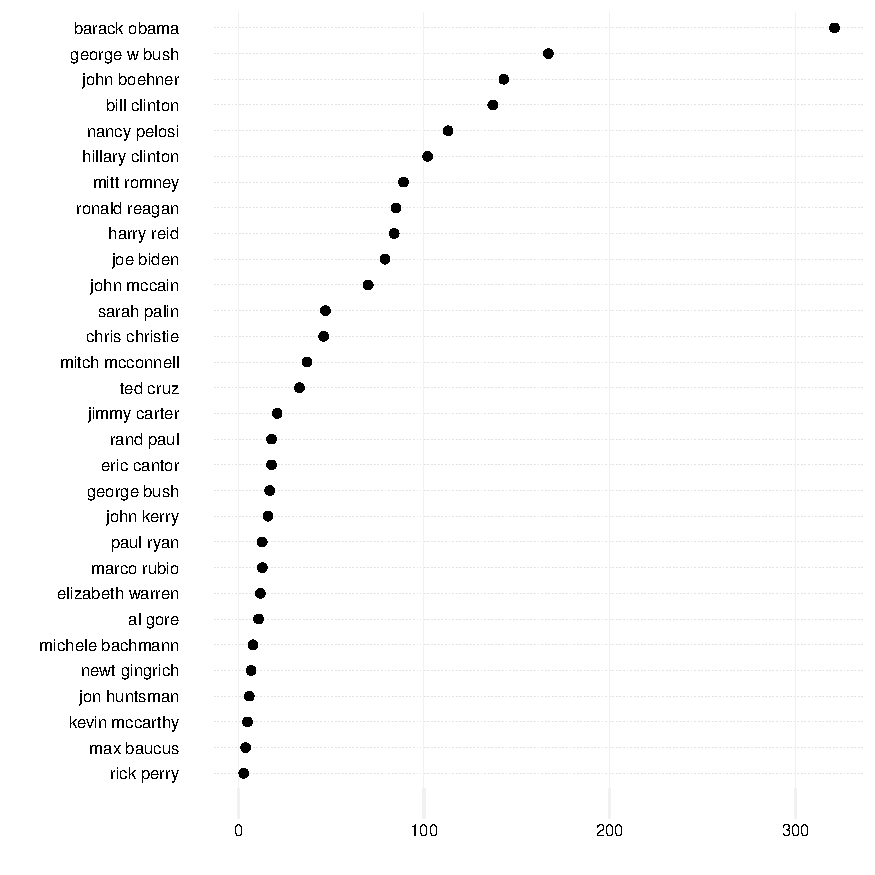
\includegraphics[width=\textwidth]{../figs/survey/names_tally.pdf}
  \label{fig:fig1}
\end{figure}


% Table created by stargazer v.5.2 by Marek Hlavac, Harvard University. E-mail: hlavac at fas.harvard.edu
% Date and time: Thu, Mar 31, 2016 - 7:44:56 PM
% Requires LaTeX packages: dcolumn 
\begin{table}[!htbp] \centering 
  \caption{Are Recalled Politicians More Extreme than the Median Senator of the Party?} 
  \label{tab:tab1} 
\begin{tabular}{@{\extracolsep{5pt}}lD{.}{.}{-3} D{.}{.}{-3} } 
\\[-1.8ex]\hline 
\hline \\[-1.8ex] 
 & \multicolumn{2}{c}{Extremity Compared to Senate Mean} \\ 
\cline{2-3} 
\\[-1.8ex] & \multicolumn{1}{c}{(1)} & \multicolumn{1}{c}{(2)}\\ 
\hline \\[-1.8ex] 
 Constant & 0.017^{**} & 0.094^{***} \\ 
  & (0.007) & (0.015) \\ 
  Out Party &  & 0.069^{***} \\ 
  &  & (0.021) \\ 
  Recall Order &  & -0.216^{***} \\ 
  &  & (0.024) \\ 
  Out Party x Recall Order &  & -0.040 \\ 
  &  & (0.034) \\ 
 \hline \\[-1.8ex] 
Observations & \multicolumn{1}{c}{1,725} & \multicolumn{1}{c}{1,725} \\ 
Akaike Inf. Crit. & \multicolumn{1}{c}{782.323} & \multicolumn{1}{c}{607.624} \\ 
Bayesian Inf. Crit. & \multicolumn{1}{c}{798.682} & \multicolumn{1}{c}{640.341} \\ 
\hline 
\hline \\[-1.8ex] 
\textit{Note:}  & \multicolumn{2}{r}{$^{*}$p$<$0.1; $^{**}$p$<$0.05; $^{***}$p$<$0.01} \\ 
\end{tabular} 
\end{table} 


\clearpage

\bibliographystyle{apsr}
\bibliography{polarnews}
\clearpage

\clearpage
\appendix
\renewcommand{\thesection}{SI \arabic{section}}
\setcounter{table}{0}\renewcommand\thetable{\thesection.\arabic{table}}
\setcounter{figure}{0}\renewcommand\thefigure{\thesection.\arabic{figure}}
\counterwithin{figure}{section}

\begin{center}
\Large{Supporting Information}
\end{center}

\section{Survey data}

Because the answers to the politician recall survey questions were open-ended (respondents typed in names), the responses were quite ``noisy'' (in addition to misspellings, some respondents just used last names, some just first names, etc) so we had to take several steps to address this.  First, we restricted attention to politicians whose exact name was used at least 3 times for at least one of the recall questions (these are the politicians listed in \ref{fig:fig1}). Then, to determine whether other respondents were attempting to refer to these politicians, we checked whether the respondent referred to the same last name (for unique last names), common misspellings of the last or first names (oboma, reed, hilary), and common stems for very difficult to spell names (boe or boh for boehner, mccon for mcconnell).  There were two non-unique last names, Bush and Clinton.  For the two Bushes: we coded any responses with 2nd, 3rd 4th or 5th word starting with s (for senior), or 2nd-3rd-4th starting with H (for middle initials H.W.) as 'george bush' and code all other responses as 'george w bush'. We coded responses of just 'clinton' as 'bill clinton'.  Regarding positions, we coded each politician as 'executive', 'legislative' or 'governor'.  We included all party nominees (president or vice president) as executive.  Failed candidates for party nomination are included in other categories.

Table ~\ref{si_survey_dem} provides a synopsis.

\begin{table}[ht]
\small
\caption{Sample Demographics Compared to Benchmarks}
\centering
\label{si_survey_dem}
\begin{tabular}{l c c c}
\hline
& Sample & 2012 ANES & 2010 Census\\
\hline
& & &\\
\textbf{Age} & & &\\
18-29 & 23.2\% & & 19.2\%\\
30-49 & 41.9\% & & 31.7\%\\
50+ & 35.0\% & & 49.2\%\\
& & &\\
\textbf{Gender} & & &\\
Male & 53.0\% & & 49.1\%\\
Female & 47.0\% & & 50.9\%\\
& & &\\
\textbf{Race/Ethnicity} & & &\\
White/Caucasian & 87.9\% & & 63.7\% \\
Black/African-American & 4.7\% & & 12.2\%\\
Asian/PI & 4.1\% & & 4.8\%\\
Hispanic/Latino & n/a \% & & 16.4\%\\
Native American & 1.0\% & & 1.1\%\\
Other/more than one & 2.2\% & & 6.2\%\\
& & &\\
\textbf{Education} & & &\\
Less than HS degree & 0.0\% & & 8.9\%\\
High school/GED & 11.1\% & & 31.0\%\\
Some college/2-year degree & 36.5\% & &28.0\%\\
4-year college degree & 41.7\% & & 18.0\%\\
Graduate/professional degree & 10.7\% & & 9.3\%\\
& & &\\
\textbf{Party Identification} & & &\\
Democratic (inc. leaners) & 56.9\% & 49.0\% &\\
Republican (inc. leaners) & 31.0\% & 39.0\% &\\
No party preference/Other & 12.2\% & 11.9\% &\\
\hline
\end{tabular}
\caption*{Note: Sample statistics are for sample used for analysis, with N=1,725 and unit of observation of (identified) recalled politician-respondent (respondents who recalled more identified politician are used more often).  White/Caucasion category is non-Hispanic for 2010 Census (no separate Hispanic category in race variable for survey).}
\end{table}
\clearpage

\subsection{Recall Results}
\label{si_recall}

% Table created by stargazer v.5.2 by Marek Hlavac, Harvard University. E-mail: hlavac at fas.harvard.edu
% Date and time: Thu, Mar 31, 2016 - 7:44:57 PM
% Requires LaTeX packages: dcolumn 
\begin{table}[!htbp] \centering 
  \caption{Estimated Extremity of Recalled Politicians} 
  \label{tab:tab1} 
\begin{tabular}{@{\extracolsep{5pt}}lD{.}{.}{-3} D{.}{.}{-3} } 
\\[-1.8ex]\hline 
\hline \\[-1.8ex] 
 & \multicolumn{2}{c}{Estimated Extremity} \\ 
\cline{2-3} 
\\[-1.8ex] & \multicolumn{1}{c}{(1)} & \multicolumn{1}{c}{(2)}\\ 
\hline \\[-1.8ex] 
 Constant & 0.790^{***} & 0.858^{***} \\ 
  & (0.007) & (0.010) \\ 
  Out Party &  & -0.104^{***} \\ 
  &  & (0.012) \\ 
  Recall Order &  & -0.058^{***} \\ 
  &  & (0.013) \\ 
  Out Party x Recall Order &  & 0.048^{***} \\ 
  &  & (0.019) \\ 
 \hline \\[-1.8ex] 
Observations & \multicolumn{1}{c}{1,715} & \multicolumn{1}{c}{1,715} \\ 
Akaike Inf. Crit. & \multicolumn{1}{c}{-977.095} & \multicolumn{1}{c}{-1,077.039} \\ 
Bayesian Inf. Crit. & \multicolumn{1}{c}{-960.754} & \multicolumn{1}{c}{-1,044.356} \\ 
\hline 
\hline \\[-1.8ex] 
\textit{Note:}  & \multicolumn{2}{r}{$^{*}$p$<$0.1; $^{**}$p$<$0.05; $^{***}$p$<$0.01} \\ 
\end{tabular} 
\end{table} 


\end{document}
